\documentclass[10pt]{article}
\usepackage{mathtools}
\usepackage{amsmath}
\usepackage{tabularx}
\usepackage{graphicx}
\usepackage{flexisym}
\usepackage{listings}
\usepackage{xcolor}
\usepackage{hyperref}
\usepackage{amsthm}
\usepackage{subcaption}
\newtheorem*{theorem}{Theorem}

\begin{document}
\setlength\parindent{1pt}
\title{Quantum Monte Carlo of confined electrons }
\author{Andrei Kukharenka and Anna Gribkovskaya \\  
FYS 4150 
}

\maketitle
\begin{abstract}
This is final project in FYS4150 course. The aim was to use Variational Monte Carlo (VMC) method to determine the ground state energy of the quantum systems. The considered system were two electrons confined in quantum dots. The quantum dot is approximated with a three-dimensional harmonic oscillator potential. Apart of ground state energy the relative distance between two electrons and expectation values of the kinetic and potential energies were evaluated. The obtained results were compared with those obtained in second project and analytical results from Taut \cite{three}. 
\end{abstract}
\clearpage 


\section{Introduction}
System under consideration is a three-dimensional harmonic oscillator potential with two electrons. Such potential trap electrons inside and prevent them to move apart. Such a trap called quantum dot and it has a large application in science \cite{four}, industry\cite{five} and medicine \cite{med}. \\
We already study such system in Project 2 using the eigenvalue solver (Jacoby method), so we are able to compare results from different methods. The advantage of VMC method is that we can use Cartesian coordinates and do not need to transform the equations. \\ 
VMC is a method for solving Schr\"{o}dinger's equation by using Metropolis sampling to simulate Markov processes. This method may seem not as straightforward as the one we used in project 2, but it is much closer to the "nature" of quantum mechanics. The quantum world is a world of probabilities and stochastic methods are much more appropriate to study the problem, even though we are limited to find only one most probable state \cite{one}. \\
All equations presented in the report are in atomic units, which means that all constants, such as speed of light or Planck's constant, are set to 1.
The report has the following structure:\\*
We begin with discussing the nature of the problem in \ref{Part1}.
In results and discussion section \ref{results} we presented all the data, plots and analysis for obtained results. 
In conclusion \ref{conc} we made a brief overview of obtained results and discuss possibilities for further research. 

\newpage
\section{Physics behind  VMC}\label{Part1}
Variational methods are widely used in quantum physics. The idea behind such method is to use some trial wave function which depend on many parameters and try to vary this parameters in order to minimize the expectation value of the energy. This method is applied in many other methods, for example the Hartree–Fock method. ADD CITATION!\\
In this project we consider simulations for the Markov chains (or random walkers). The essence of such process is that it depend only on a previous move and do not have "memory" about the all previous.


As all other variational methods the VMC uses the so-called trial functions. 




\newpage
\section{Results and discussion}\label{results}

In this project we start with non interacting system. We use first trial wave function to determine the optimal value of variational parameter $\alpha$ and also to check the result against the one we got analytically in the section above. From \ref{fig:fig1} one can see that the optimal variational parameter $\alpha$ for this case is 1. In Table \ref{tab:one} we presented the mean distance at the energy minimum for the first trial wave function. As one can see from the table the mean distance between two electrons become bigger as the harmonic oscillator strength $\omega$ decreases. \\
ADD EXPLANATION!!!!

\begin{table}[h!]
  \caption{Relative distance between two electrons for different values of $\omega$. Variational parameter $\alpha =1$}
  \label{tab:one}
  \begin{center}
    \begin{tabular}{c|c|c}
    \hline
		$\omega$& Expectation Energy & Expectation relative distance \\
    \hline
	$	1 $  & $3.0$ & $1.5964$  \\
	$	0.5$  & $1.5$ & $2.2565$   \\
	$	0.01$  & $0.03$ &  $15.977$   \\
	\end{tabular}
  \end{center}
\end{table}




\begin{figure}[h!] 
  \begin{subfigure}[b]{0.6\linewidth}
    \centering
    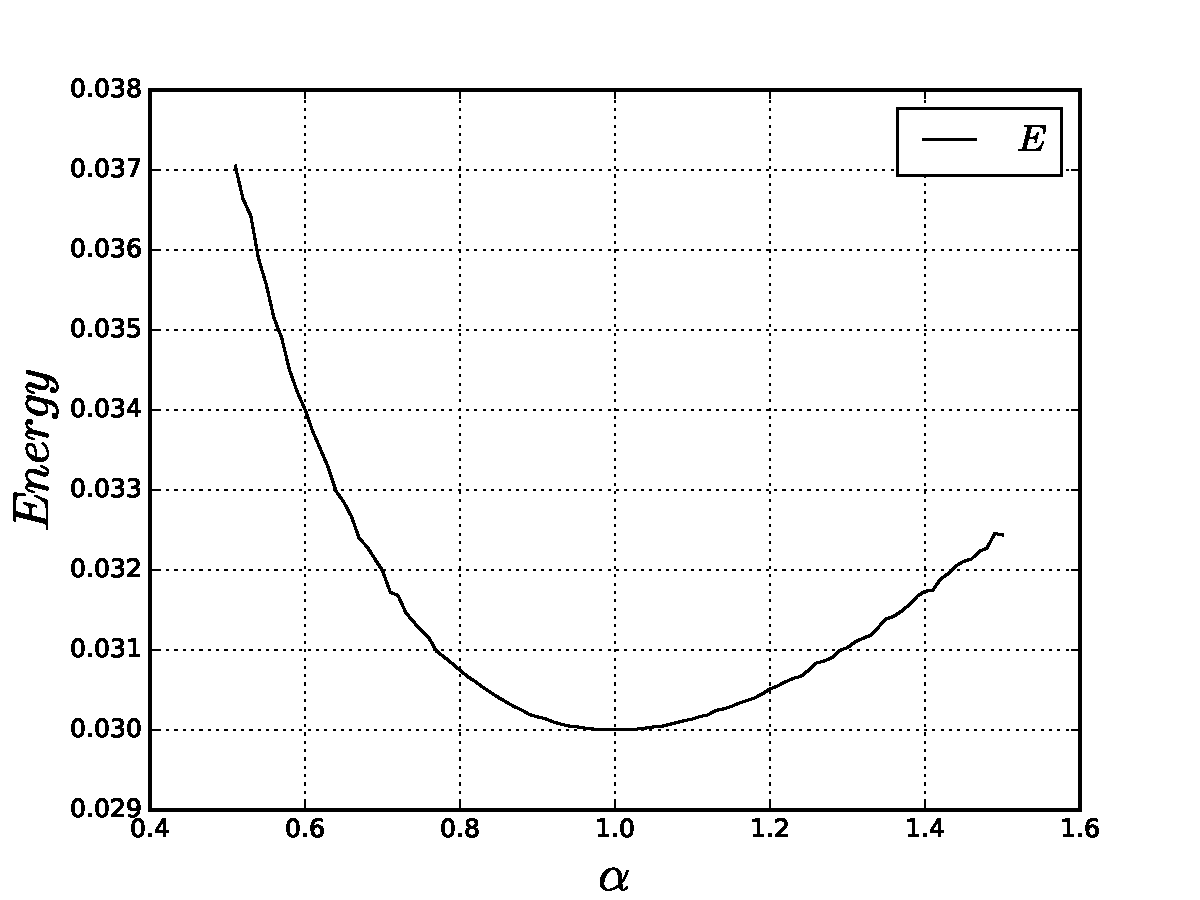
\includegraphics[width=1.1\linewidth]{energy_on_alpha_001} 
    \caption{The $\omega$ is 0.01} 
    \label{fig1:a} 
    \vspace{1ex}
  \end{subfigure}%% 
  \begin{subfigure}[b]{0.6\linewidth}
    \centering
    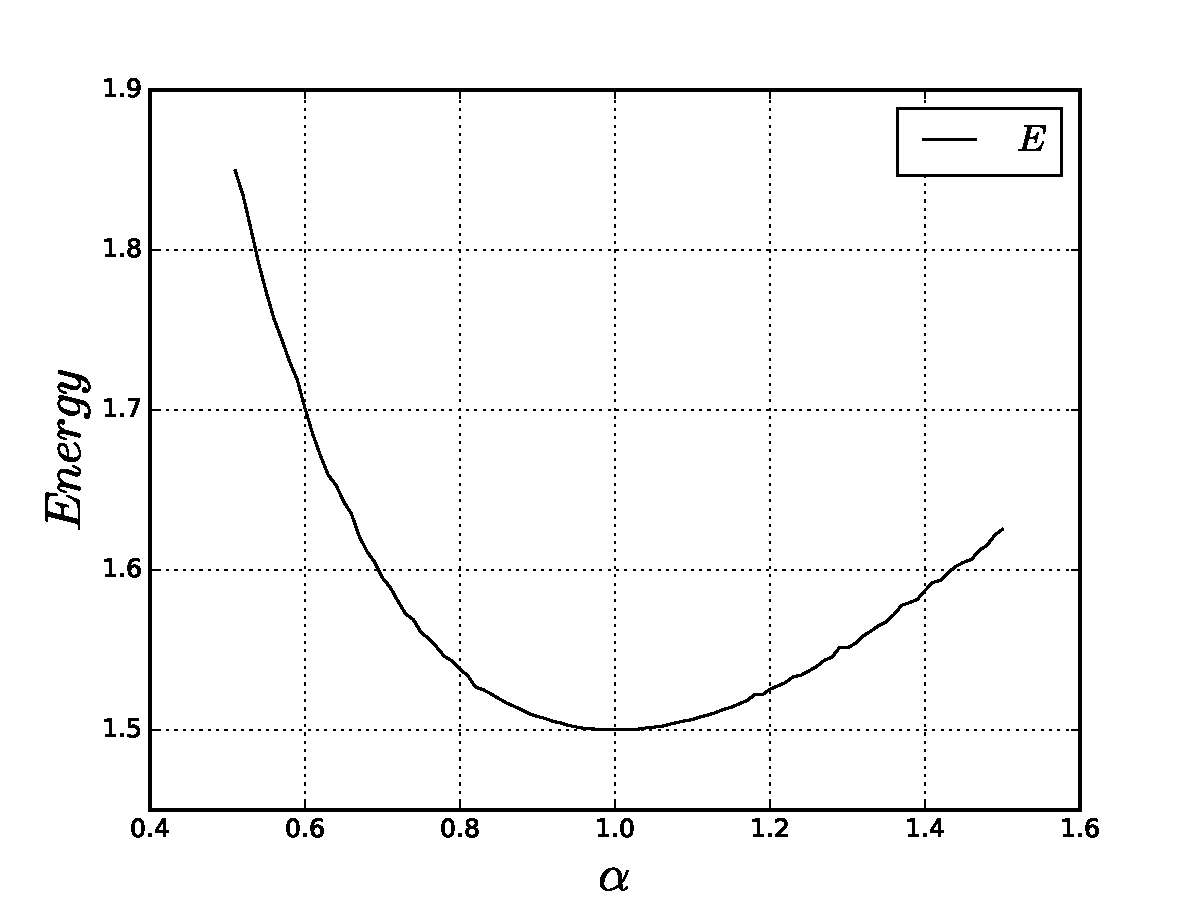
\includegraphics[width=1.1\linewidth]{energy_on_alpha_05} 
    \caption{The $\omega$ is 0.5} 
    \label{fig1:b} 
    \vspace{1ex}
  \end{subfigure} 
  \begin{subfigure}[b]{0.6\linewidth}
    \centering
    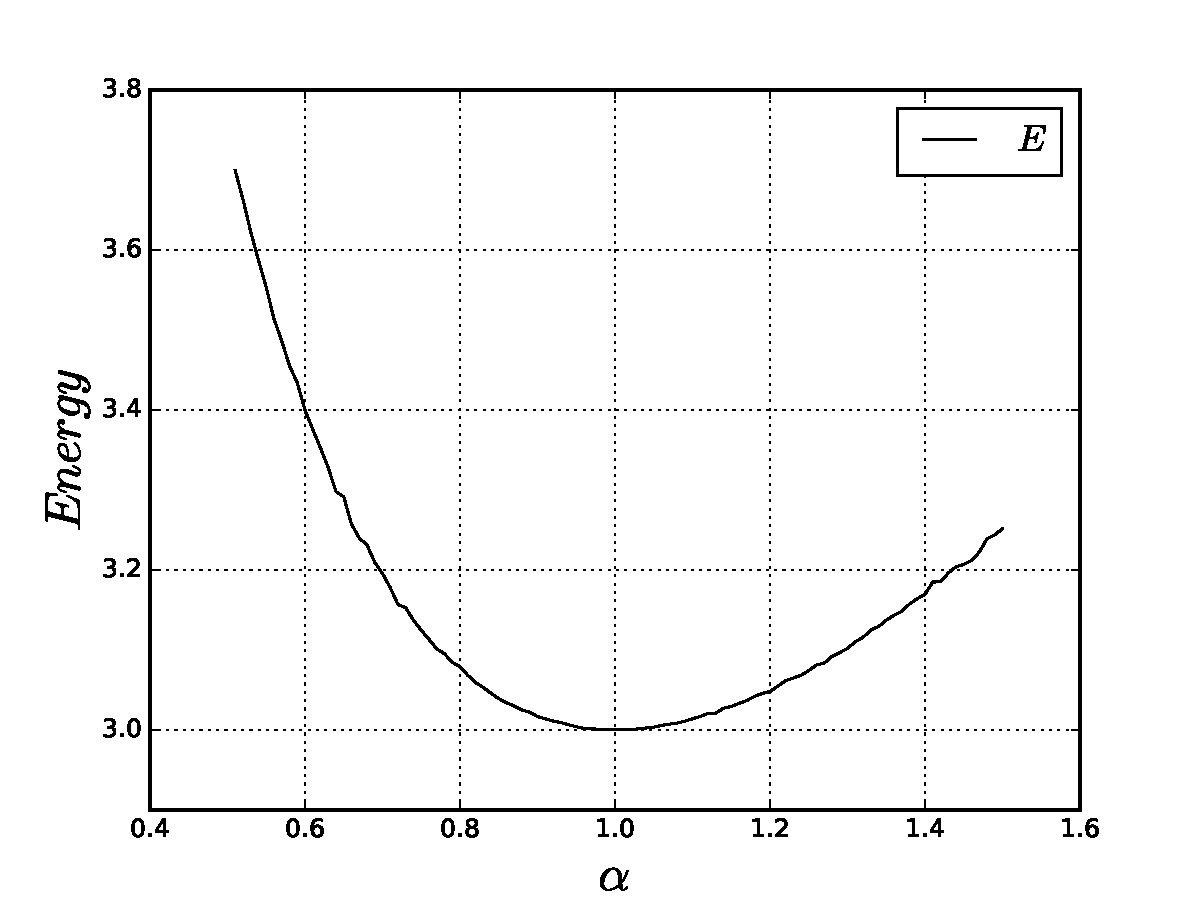
\includegraphics[width=1.1\linewidth]{energy_on_alpha_1} 
    \caption{The $\omega$ is 1} 
    \label{fig1:c} 
  \end{subfigure}%%
  \begin{subfigure}[b]{0.6\linewidth}
    \centering
    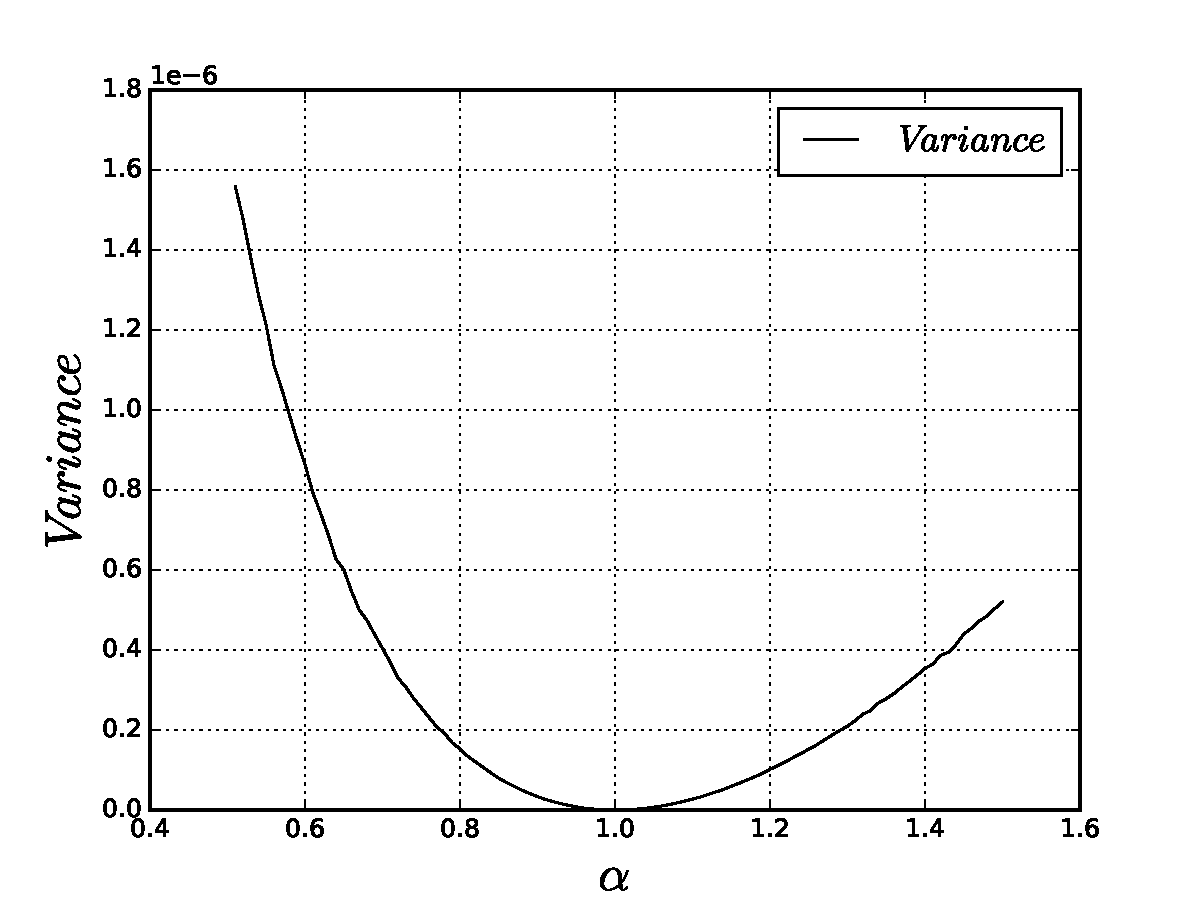
\includegraphics[width=1.1\linewidth]{variance_on_alpha} 
    \caption{The $\omega$ is 1} 
    \label{fig1:d} 
  \end{subfigure} 
  \caption{ Energy a)to c) and energy variance d) as a function of variational parameter $\alpha$.}
  \label{fig1} 
\end{figure}

The second trial wave function depend on two parameters $\alpha$ and $\beta$. In this case we need to vary both parameters and fin the minimal energy. All results are presented in Table \ref{tab:two}.

\begin{table}[h!]
  \caption{Relative distance between two electrons and minimal energy for different values of $\omega$.Variational parameters are $\beta = 0.355$ and $\alpha = 0.9845$}
  \label{tab:two}
  \begin{center}
    \begin{tabular}{c|c|c}
    \hline
		$\omega$ & Expectation Energy & Expectation relative distance \\
    \hline
	$	1 $  & $3.73094$ & $2.46374$  \\
	$	0.5$  & $2.00473$ & $2.61461$   \\
	$	0.01$  & $0.100629$ & $41.0782$   \\
	\end{tabular}
  \end{center}
\end{table}


\newpage
\clearpage
\section{Conclusion and further research}\label{conc}


\clearpage
\newpage

\begin{thebibliography} {9}
\bibitem{three}
M. Taut. 
\textit{Two electrons in an external oscillator potential: Particular analytic solutions of a Coulomb correlation problem}.
Phys. Rev. A, 11.1993.


\bibitem{four}
D. Loss, D. P. DiVincenzo
\textit{
Quantum computation with quantum dots
}
Phys. Rev. A 57, 120 – Published 1 January 1998.

\bibitem{five}
P. Patel
\textit
{The First Full-Color Display with Quantum Dots
}
MIT Technology Review, February 22, 2011.

\bibitem {med}
Yuri Volkov
\textit
{Quantum dots in nanomedicine: recent trends, advances and unresolved issues
}
Biochemical and Biophysical Research Communications, Volume 468, Issue 3, 18 December 2015, Pages 419–427

\bibitem{one} 
Morten Hjorth-Jensen. 
\textit{Computational Physics
}. 
Lecture Notes Fall 2015, August 2015.
\bibitem{two} 
W. Press, B. Flannery, S. Teukolsky, W. Vetterling 
\textit{Numerical Recipes in C++, The art of scientific Computing}. 
Cambridge University Press, 1999.


\bibitem {wigner}
E.P. Wigner
\textit
{On the interaction of electrons in metals
}
Phys. Rev. B 46, 1002 (1934) 

\bibitem {log}
Ed S. Coakley, V. Rokhlin
\textit
{A fast divide-and-conquer algorithm for computing the spectra of real
symmetric tridiagonal matrices
}
Appl. Comput. Harmon. Anal. 34 (2013)

\end{thebibliography}

\end{document}
